% 第5章第4节：树分解与树宽（袋与接口、树分解的三个条件、团必被某袋容纳、宽度与树宽）。

\section{树分解与树宽}
\label{sec:graph-tree-decomposition}

上一节看到，变量消元的开销取决于每一步同时处理的变量组。本节把这些变量组单独拿出来，研究它们怎样组织成一棵树，才能让计算沿树进行而不丢失一致性。先从消元过程引出“袋”和“接口”，再给出合法分解的三个条件，最后用袋的大小定义宽度和树宽。本节只讨论结构本身：怎样构造分解放在第~\ref{sec:graph-tree-decomposition-construction}节，怎样在分解上计算放在第~\ref{sec:graph-bag-dp}节。

\subsection{袋与接口}

\paragraph{从消元步骤到袋}
回到四变量例子的次序$(1,4,2,3)$。消去$x_1$时要同时处理$\{1\}\cup R_1=\{1,2,3\}$，消去$x_4$时处理$\{2,3,4\}$，随后依次处理$\{2,3\}$和$\{3\}$。每一步产生的新函数会在后面某一步被用到：$\psi_1$与$\psi_4$都在消去$x_2$时被合并，$\psi_2'$在消去$x_3$时被使用。把每一步同时处理的变量集合看成一个节点，按“新函数交给哪一步使用”连接这些节点，就得到图~\ref{fig:graph-dp-bags-interface}中间的一棵树。

这种准备放进同一张表里同时索引的变量集合称为\term{袋}（bag），袋组成的树称为袋树。袋树的节点是计算单元，袋树的边表示两个计算单元之间传递一张表；它与原始图中连接两个变量的边含义不同。不同的袋可以有公共变量，例如$\{1,2,3\}$与$\{2,3,4\}$都含$2,3$。

\begin{figure}[!htb]
  \centering
  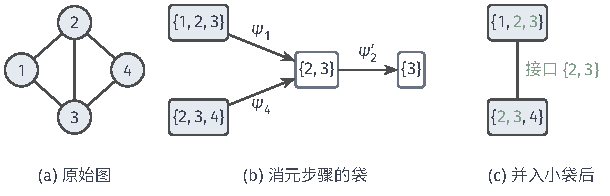
\includegraphics[width=103.283mm]{figures/01-basic-mathematics/04-graphs/tikz/c5-elimination-to-bags/figure.pdf}
  \caption{从消元步骤得到袋。左：四变量例子的原始图。中：按次序$(1,4,2,3)$消元时，每一步同时处理的变量集合构成一个袋，箭头表示新函数交给哪一步使用。右：$\{2,3\}$和$\{3\}$已包含在相邻的大袋中，并入后只剩两个袋，它们的交集$\{2,3\}$（绿色）就是接口。}
  \label{fig:graph-dp-bags-interface}
\end{figure}

袋与原始图中的“团”有关，但不必是团。原始图中两两相邻的顶点集合称为\term{团}（clique）。四变量例子中$\{1,2,3\}$是团，$\{1,2,4\}$不是，因为缺边$\{1,4\}$。按次序$(2,1,3,4)$消元时，第一步要同时处理$\{1,2,3,4\}$，这个袋在原始图中不是团，只在补入填充边后才成为团。所以袋可以重叠，也可以含有原图中不相邻的变量。

\paragraph{接口}
袋$\{2,3\}$和$\{3\}$都已包含在相邻的大袋中，可以并入，最后只剩两个袋$\{1,2,3\}$与$\{2,3,4\}$，如图~\ref{fig:graph-dp-bags-interface}右侧。相邻两袋的交集称为它们的接口（interface），这里是$\{2,3\}$。接口上的变量在两个袋里是同一个变量，不是两个副本：左袋在汇总$x_1$时必须对$(x_2,x_3)$的每种取值分别给出结果，右袋使用这些结果时也必须按同样的$(x_2,x_3)$取值来读。左袋的结果正是$\psi_1(x_2,x_3)$，一张以接口为索引的表。

由此提出一个要求。若某个变量出现在两个不相邻的袋中，而连接它们的袋树路径上有某个袋不含这个变量，那么两侧的计算无法通过接口约定这个变量取同一个值。为了让每个变量的取值在它出现的所有袋之间保持一致，袋的连接方式必须受到限制。下面把这个要求与覆盖要求一起写成定义。

\subsection{树分解的条件}

\paragraph{三个条件}
袋必须能容纳所有局部函数，袋之间的连接又必须保证一致。结构上，前一项要求每个变量和原始图的每条边都被某个袋包含，后一项就是上面提出的连接要求。

\begin{definition}[树分解]
\label{def:graph-dp-tree-decomposition}
设$\mathcal G=(V,E)$是有限无向图。$\mathcal G$的一个\term{树分解}（tree decomposition）由一棵有限树$\mathcal T$（节点集记为$T$）和每个节点$t\in T$上的子集$B_t\subseteq V$组成，满足：
\begin{enumerate}
  \item 顶点覆盖：每个顶点$v\in V$至少属于一个袋；
  \item 边覆盖：对每条边$\{u,v\}\in E$，存在某个袋同时含有$u$与$v$；
  \item 运行交集：对每个顶点$v\in V$，含$v$的节点集合$T_v=\{t\in T:v\in B_t\}$在$\mathcal T$中连通。
\end{enumerate}
第三个条件称为\term{运行交集性质}（running intersection property）。
\end{definition}

运行交集等价于：若$v$同时属于$B_s$和$B_t$，则$\mathcal T$中从$s$到$t$的路径上每个袋都含$v$。因为树中两点之间只有一条路径，$T_v$连通恰好意味着这条路径留在$T_v$中。

\paragraph{只覆盖边还不够}
图~\ref{fig:graph-dp-running-intersection}比较路径$1-2-3-4$上的两种袋连接。两种连接使用同样的三个袋$\{1,2\},\allowbreak\{2,3\},\allowbreak\{3,4\}$，都覆盖了全部顶点和边。上面一种按$\{1,2\}-\{2,3\}-\{3,4\}$连接，含$2$的两个袋相邻，含$3$的两个袋也相邻，是树分解。下面一种按$\{1,2\}-\{3,4\}-\{2,3\}$连接，含$2$的两个袋被不含$2$的袋$\{3,4\}$隔开。若沿这棵树计算，左端的袋可以选$x_2=0$，右端的袋可以选$x_2=1$，中间的袋不记录$x_2$，无从发现矛盾；拼起来的结果不对应任何一个配置。

\begin{figure}[!htb]
  \centering
  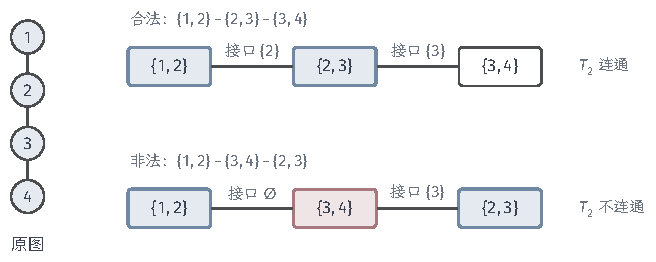
\includegraphics[width=111.016mm]{figures/01-basic-mathematics/04-graphs/tikz/c5-running-intersection/figure.pdf}
  \caption{路径$1-2-3-4$上的合法与非法袋连接。两种连接使用相同的三个袋，都覆盖全部顶点和边。上：含$2$的袋（蓝色）彼此相邻，含$3$的袋也相邻，满足运行交集。下：含$2$的两个袋之间隔着不含$2$的袋$\{3,4\}$（红色），$T_2$不连通，不是树分解。}
  \label{fig:graph-dp-running-intersection}
\end{figure}

\paragraph{完整作用域总能放进某个袋}
计算时每个局部函数要整个放进一个袋，因为袋表需要同时索引它的全部变量。一个作用域$S_a$在原始图上是团：其中任意两个变量同在$\phi_a$中，因而相邻。但树分解的定义只要求每条边被某个袋覆盖，三个变量两两成边时，三条边可能分别落在三个不同的袋中。下面的引理说明这种情况不会发生。

把每个顶点$v$的出现位置$T_v$看成袋树中的一棵连通子树。若$u,v$相邻，边覆盖给出一个同时含$u,v$的袋，于是$T_u$与$T_v$相交。对一个团$C$，各$T_v$（$v\in C$）两两相交；要证明的是它们有一个公共节点。

\begin{lemma}[团被某个袋容纳]
\label{lem:graph-dp-clique-in-bag}
设$(\mathcal T,\{B_t\}_{t\in T})$是$\mathcal G$的树分解，$C\subseteq V$是$\mathcal G$中的非空团，则存在节点$t\in T$使$C\subseteq B_t$。
\end{lemma}

\begin{proof}
任取袋树的一个节点作为根。对每个$v\in C$，$T_v$非空且连通。先说明$T_v$中有唯一一个离根最近的节点，记为$r_v$，并且$T_v$的每个节点都是$r_v$的后代（含$r_v$本身）。若$y\in T_v$不是$r_v$的后代，从$y$到$r_v$的树上路径要先向上经过$y$与$r_v$的最近公共祖先$z$，而$z$比$r_v$更靠近根；由$T_v$连通，这条路径留在$T_v$中，于是$z\in T_v$，与$r_v$的选取矛盾。同样的论证也说明离根最近的节点唯一。

在$C$中取一个顶点$w$，使$r_w$的深度在$\{r_v:v\in C\}$中最大。下面证明$r_w$属于每个$T_u$（$u\in C$）。$u=w$时，$r_w\in T_w$由定义成立。$u\neq w$时，$u,w$相邻，所以$T_u\cap T_w$中有某个节点$x$；$x\in T_w$，因而$x$是$r_w$的后代。考察$T_u$中从$x$到$r_u$的路径，它留在$T_u$中。若$r_u$不是$r_w$的后代，这条路径从$r_w$子树内部走到外部，必须经过$r_w$，于是$r_w\in T_u$。若$r_u$是$r_w$的后代，则$r_u$的深度不小于$r_w$的深度；而按$w$的选取，$r_u$的深度又不大于$r_w$的深度，所以$r_u=r_w$，同样有$r_w\in T_u$。因此$r_w$属于全部$T_u$，袋$B_{r_w}$含有整个$C$。
\end{proof}

图~\ref{fig:graph-dp-clique-in-bag}画出了证明中的几棵子树：每个变量的出现位置向上延伸到自己的最高节点，最高节点最深的那个变量，它的最高节点被其余各子树“经过”，因而就是要找的袋。

\begin{figure}[!htb]
  \centering
  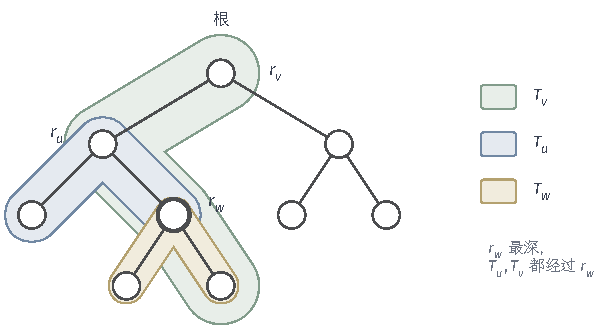
\includegraphics[width=102.648mm]{figures/01-basic-mathematics/04-graphs/tikz/c5-clique-in-bag/figure.pdf}
  \caption{团$\{u,v,w\}$被某个袋容纳的论证。袋树以顶部节点为根，三种颜色的区域分别是$T_u$、$T_v$、$T_w$，标签$r_u,r_v,r_w$标出各自离根最近的节点。$r_w$最深；$T_u$、$T_v$都要与$T_w$相交，而它们的最高节点不比$r_w$深，所以必须经过$r_w$。粗圈节点$r_w$的袋同时含$u,v,w$。}
  \label{fig:graph-dp-clique-in-bag}
\end{figure}

由引理~\ref{lem:graph-dp-clique-in-bag}，原始图的任一树分解中，每个局部函数的完整作用域都被某个袋整体容纳。因此在原始图上构造树分解就足够了，不需要额外记录高阶作用域；第~\ref{sec:graph-local-functions}节所说的“结构以原始图为依据、计算保留完整函数”在这里得到保证。

\subsection{宽度与树宽}

袋越大，袋表越大。为了用一个数概括一次分解的规模，定义树分解的宽度为$\max_{t\in T}|B_t|-1$，即最大袋的大小减一；图$\mathcal G$的\term{树宽}（treewidth）是它的全部树分解宽度的最小值，记为$\operatorname{tw}(\mathcal G)$。减一是一种约定，使得下面的树恰好宽度为一。

\paragraph{三个小例子}
单个顶点的图只需一个袋$\{1\}$，宽度为$0$，任何没有边的图都如此。至少含一条边的树宽度为$1$：任选根$\rho$，为每个非根顶点$u$建袋$\{u,p(u)\}$，其中$p(u)$是父点；若$p(u)$不是根，就把这个袋连到$p(u)$自己的袋上，根的各子点的袋则依次连成一条链。这样，非根顶点$v$出现在自己的袋和各子点的袋中，后者都与前者相邻；根只出现在各子点的袋中，它们连成链，所以运行交集成立。另一方面，一条边要求某个袋含两个顶点，宽度不能小于$1$。

四个顶点的环$1-2-3-4-1$有宽度为$2$的树分解：两个袋$\{1,2,3\}$与$\{1,3,4\}$，以一条边相连，接口为$\{1,3\}$。它没有宽度为$1$的树分解。证明沿用引理~\ref{lem:graph-dp-clique-in-bag}的思路：给任一树分解选根，在环上取$w$使$r_w$最深，$w$在环上的两个邻居$u,v$各自与$w$相邻，于是$T_u$、$T_v$都与$T_w$相交，上面的论证表明$r_w\in T_u\cap T_v$。这个袋含$u,v,w$三个顶点，所以宽度至少为$2$。这一论证对任何环都适用：含环的图树宽至少为$2$，树宽为$1$的图恰好是至少含一条边的森林（森林的各个分量分别按上面的方法分解，再用任意的边把各分量的袋树连成一棵树；不同分量没有公共顶点，这些连接不影响运行交集）。

这几个例子说明，树宽衡量的是图与树的接近程度：一条边需要两个变量同时出现，一个环则迫使某处至少三个变量同时出现。还要注意，某一次构造得到宽度$k$，只说明$\operatorname{tw}(\mathcal G)\leq k$；要断言树宽恰为$k$，还需要像上面那样证明不存在更小宽度的分解。

\paragraph{宽度与表的大小}
若每个变量至多有$q$个状态，宽度为$k$的分解中，每个袋至多有$k+1$个变量，稠密存储的袋表至多$q^{k+1}$项。这是第~\ref{sec:graph-bag-dp}节中主要的枚举规模。实际的总开销还包括袋的个数、接口的大小和每次读取局部函数的成本，宽度只控制其中随状态数指数增长的那一部分。

最后，寻找树宽最小的分解与使用一个已经给定的分解是两项不同的任务。前者在一般图上是困难的组合问题；后者只需检查三个条件并沿树计算。第~\ref{sec:graph-tree-decomposition-construction}节给出的构造方法都只保证得到合法的分解和宽度上界。
